


\section{Dream}

The increasing trend of digitisation and the ensuing ubiquity of personal data in the cloud touch on sensitivities more than ever before. 
In response to the former, regulators often formulate requirements on removability that fails to recognise 
that it is virtually impossible to make material once seen become unseen.
Entities that operate infrastructure underpinning digital publishing are in control of the technology serving the content and  are able to implement "removal" by denying access.
Such centralised gate-keeping  has its regulatory appeal as it can be thought of as an instrument of law enforcement. Although such intervention rarely solves the breach of unrealistic privacy rights, the gate-keeper provides a well-defined responsible party with the effective course of action: not serving censored content.
While this gives the unwary a phony sense of security, it only exemplifies the bigger problem of censorship: publishing platforms have the technological means to filter content and centralised control makes exerting influence on content cheaper.  What starts out as sensible measures of content curation with time becomes extant censorship. This is all the more problematic with social platforms that gained quasi-monopolistic status due to netwtork effects. As a result of high switching cost, innocent content creators ever more often end up being 'deplatformed'. Similarly, the ability to identify hosts and deny access to content via legal decree gives powers to be the means to infringe on freedom of speech. 

In the decentralised paradigm of web 3, there is no longer an operating entity behind either the publishing platform or the hosting infrastructure. Therefore, the cost of censorship is raised beyond the realm of feasibility. And yet, the potential permanent exposure of personal data is perceived as scary to most and some novel solution is called for to restore the sense of security gate-keepers purportedly represent. 

\subsection{Deletion and revoking access}

First, notice that any reference to removal of information in the sense of erasing it from all physical storage devices is both unenforceable and impractical. Even the strictest data protection audits do not require the erasure of offending data from backup tapes. In general, the tacit assumption is that information ordered to be removed should become inaccessible through \emph{typical precedented methods of access}.

In what follows we formulate the strongest meaningful definition of deletion applicable to decentralised storage and offer a construction that implements it.
Importantly, such a construction is purely technical, referring to primary actors' capabilities and costs as opposed to procedural, referring to intermediaries' obligations to respect the rights of primary actors. 

Primary actors here are the \emph{uploader} that wishes to share content by granting read access to a number of parties, called \emph{downloaders}.  Granting access is defined as providing some canonical \emph{reference} to the content that the system can eventually resolve to the full information meant to be disclosed. Any party that is privileged to access this information, is able to store, re-code and potentially disseminate it. This provides a myriad of ways to make accessible the content at any later point in time to get round whatever process would qualify as deletion or removing access. 
There is, by definition, no protection possible against such adversity. As a consequence, any legally sound notion of deletion (retrospective revocation of access) is meant to be interpreted in a narrower sense: \emph{the viability to replay the same access method}  for a cost lower than the \emph{full cost} of storing the content.%
%
\footnote{That is, the total cost of storage paid for the full size for the entire period kstarting from the time access was revoked uptill the attempted breach.}

Let us now define deletion as a scheme for uploading content with access revocation that has the following requirements: 

\begin{itemize}[noitemsep]
    \item[--] \emph{specialisation} -- Uploader is able to choose at the time of publishing a specialised construct%
%
\footnote{From a user's perspective, content that is meant to be reliably deleted should be uploaded as such. The costs of uploading such content is allowed to be a (small integer) multiple of the cost of regular, censorship-resistant but non-deletable uploads.}
%
    allowing retrospective revocation of access.
    \item[--] \emph{sovereignty} -- Uploader is the sovereign owner of the data and is in sole possession of the means to selectively revoke access from any party previously granted access.%
%
\footnote{The uploader's credentials are necessary to delete their own deletable content. Deletables must also allow access control, i.e., only available to a specific set of recipients.}
%
    \item[--] \emph{security} -- After revocation of access, a grantee is unable to access the content using the same reference that the access was granted with, or any other cue shorter than the deleted content.%
%
\footnote{In other words, if the downloader has \emph{not} stored at least as much information as the deleted information itself, they will have no way of retrieving it.}
%
\end{itemize}

Note that normally uploaded content may be \emph{forgotten}: if nobody pays for storing it and it is not accessed sufficiently often, the chunks constituting it will be garbage collected. However, chunks with  expired postage stamps cannot be regarded as reliably deleted to satisfy the requirements of sovereignty and security. 


\subsection{Construction}

The goal of this section is to arrive at a formal construction of a DISC-based revocable access model. We will restrict our scheme to \emph{chunks}, the fundamental fix sized storage unit of Swarm's DISC model.  The proposed \emph{dream} construct implements a  deletable content storage and access model conforming to the requirements of specialisation, sovereignty, and security. The use of the word 'dream' alludes to the somewhat unexpected finding that such a construct is even possible in the immutable DISC model. On top of this, as customary in swarm, it serves as a mnemonic acronym, resolving to the 5 \emph{dream attributes} expressing requirements of access control.

\begin{itemize}
    \item[\textbf{D}] \emph{deniable} -- the dream key serves as a one time pad for decryption. Since multiple content chunks (in fact any arbitrary content) can use the same dream pad, the key's association to any content is plausibly deniable.
    \item[\textbf{R}] \emph{revocable} -- access granted by dream keys is revocable. Revoking access from all parties including oneself is taken as deletion.   
    \item[\textbf{E}] \emph{expirable} -- the scheme allows for one-time use, i.e., the key can only be retrieved once.
    \item[\textbf{A}] \emph{addressable} -- access can be granted to a neighbourhood, only clients operating a node with an overlay address in a given range  are able to access.
    \item[\textbf{M}] \emph{malleable}  --  the construct is resilient to churn and dynamic change of network size, is reusable across independent grantees and upgradeable.
\end{itemize}

The scheme is built on top of DISC's APIs and can be implemented entirely as a second layer solution.  Despite its rich feature set, the scheme does not use complex cryptography, but relies on the interplay of various component subsystems.

% The network protocols of Swarm use forwarding Kademlia  meaning that requests are routed to their destination through a series of hops successively relayed by forwarding nodes with ever increasing proximity to the target address.

% The chunk delivery to storer nodes can also be seen as a request: the closest node respond with a statement of custody that is passed back via the same route as the original request (\emph{backwarding}). 

% \subsubsection{Pseudo-random sequence from generator}

Assume we have a pseudo-random deterministic function that generates a longer (e.g., chunk-sized = 4K) sequence $c$ from a key-sized (32 byte) generator $g$.%
%
\footnote{For example, the Keccak sponge function used throughout Ethereum for hashing does have this capability. Alternatively, the blockcipher encryption using initial nonce $g$ could be applied to a  fixed constant chunk such as all zeros.}

% \subsubsection{Dream: deniable, revocable, expirable, addressable, malleable}

The central construct called a \emph{dream} is a chunk-sized one time pad which acts as a decryption key for the deletable content. The dream chunk is collectively created by a set of nodes following a network protocol. Each node in the sequence of participating peers receives a piece of data and uses it as input together with data present in their reserve to produce an output sent to the neighbourhood of the next node in the chain. As long as each node in the chain performs the same calculation and forwards the same result, the same one time pad can be construed and ultimately the deletable content can be retrieved and read.

The insight here is that retrieving a deletable chunk's references involves calculations using a set of immutable chunks under the control of the uploader. The uploader's ability to change this underlying set holds the key to providing the necessary mutability required by any notion of deletion. 
 
Let $b$ be the batch ID (a 32-byte hash) of a postage batch owned by $U$ and 
let $\mathit{Chunks}(\gamma,b,p)$ stand for all chunks stamped by $b$ at block $\gamma$ in the bucket designated by the pivot $p$. Define  $\overline{\Huge\chi}(\gamma,b,p)$ as the chunk stamped by batch $b$ in bucket designated by $p$ older than $\gamma$  whose address is closest (has minimal XOR distance) to pivot $p$.

\begin{eqnarray}
\overline{\Huge\chi}&:& \Gamma\times\mathit{Batches}\times \mathit{Segment} \mapsto \mathit{Chunks}\\
\overline{\Huge\chi}(\gamma,b,p)&\defeq &\underset{c\in \mathit{Chunks}(\gamma,b,p)}{\operatorname{arg\,min}}{\Large\chi}(p,\textsc{Address}(c))
\end{eqnarray}

If batch $b$ is underutilised, a bucket designated by $p$
may not contain any chunks belonging to the batch bucket.
In such cases there is no chunk closest to $p$, thus the \emph{BBB} function is undefined.

Let us now define the OTP update function $\Delta(\gamma,b)$
for batch ID and input address $p$ as follows: 
%
\begin{eqnarray}
{\Delta}&:&\Gamma\times\mathit{Batches}\mapsto\mathit{Chunks}\mapsto\mathit{Chunks}\\\
{\Delta}(\gamma, b)&:&\mathit{Chunks}\mapsto\mathit{Chunks}\\
\Delta(\gamma,b)(c)&\defeq&\mathcal{G}\idx{4K}(\textsc{Address}(\overline{\Huge\chi}(\gamma,b,c)))
\end{eqnarray}


Since uniformity depth of batches is meant to be larger than nodes' storage depth, all chunks in a batch bucket designated with $p$ is  in the reserve of every node in the neighbourhood designated by $p$. 

If swarm grows and  there are nodes whose storage  depth is higher than the batch's uniformity depth, then the neighbourhood designated by $p$ may not contain all the
chunks in the bucket, thus compromising the computability of the OTP update function.

As long as 1) the bucket of batch $b$ designated by $p$ is not empty and 2) the neighbourhoods include (one or more) buckets then the update function is computable by any storer node within the neighbourhood designated by $p$.

Since the task function can be applied to its own output, we can define \emph{dream path}:


\begin{eqnarray}
\Pi(b,g)&\defeq&c_0,\ldots, c_n\in\mathit{Chunks}\{n\}\\
c_i&\defeq&\begin{cases}
\mathcal{G}\idx{4K}(g) &\text{if }i=0\\   
\Delta(b,c_{i-1}) &\text{otherwise}
\end{cases}
\end{eqnarray}

The dream path function is a pseudo random generator defined by finite recursion. A \emph{dream} is a particular pairing of a generator and a one time pad that are input and output of a dream path.
Given a dream path of length $n$ and grantee overlay address $a$ and a batch $b$ with uniformity depth $d$, uploader needs to find the generator $g$, such that the $n$-th chunk of the dream path should land in $a$'s neighbourhood (i.e., $\mathit{PO}(a,\textsc{address}(c_{n-1}))\geq d$).

\begin{eqnarray}
\mathit{dream}(b,n,a) &\subset &\mathit{Keys}\times\mathit{Chunks}\\
\langle g, k\rangle &\in& \mathit{dream}(b,n,a) \\
&&\Longleftrightarrow\\
&&k=\Pi(b,g)\idx{n}
\land\\
&&\mathit{PO}(a,H_{\mathit{bmt}}(k))\geq d
\end{eqnarray}

The uploader is able to construct the dream pad.
As a result they can also calculate $k$ given $g$. Since $\mathit{H}(k)$ is uniform, the chance of $\mathit{PO}(a,\mathit{H}(k))\geq d$ is 1 in $2^{d}$. 



Now we can turn to the definition of a dream, a network protocol based access method that is deniable, revocable, expirable, addressable, malleable. In order for downloaders to calculate the dream pad, they must rely on the network, whereby each recursive step is calculated by a node in the neighbourhood designated by the respective input chunk's address. 

In order to guarantee the correct termination, the following criteria must be fulfilled:
\begin{itemize}[noitemsep]
\item[---] all  buckets of batch $b$ designated by $p_0,\ldots, p_{n-1}$ amust be non-empty
\item[---] uniformity depth of the batch must remain higher than the storage depth of nodes in the neighbourhoods designated by $p_0, \ldots , p_{n-1}$.
\item[---] the output of each step produced by a node in the neighbourhood designated by $p_i$ must be sent to the 
neighbourhood designated by $p_{i+1}$. 
\item[---]  nodes in the neighbourhoods on each hop of the dream path (designated by $p_0,\ldots, p_{n-1}$) must be 
incentivised to compute the OTP update as well as send off the resulting output chunk to the next neighbourhood. \end{itemize}


\begin{figure}[htbp]
  \centering
    % \includegraphics[width=0.8\textwidth]{}
  \caption{The dream protocol}
\label{fig:protocol}
\end{figure}


Let us  define a network protocol \emph{dream} (see figure \ref{fig:protocol}). Those who play the protocol, listen to single owner chunks wrapping the input.
We assume that they extract the batch identifier $b$, and the payload CAC $c$ as parameters to the OTP update function and then calculate the output pad, wrap it as a dream chunk and send it to the network towards the address of the output chunk so that the destination neighbourhood 
can calculate the next step. If the protocol is followed up to $n$ steps, then $k=c(n)$ is received by the target node at address $a$. 


We now turn to the construction of dream chunks. 
Uploader $U$ wishes to grant downloader $D$ (at overlay address $a$) revocable  access to content chunk $C$.
$U$  chooses a postage batch $b$ it owns that is completely filled, a step-count $n$, and a depth $d$.
$U$ creates a dream generator $\langle g, k\rangle\in\mathit{dream}(b,d,n,a)$.              

$U$ calculates the "ciphertext" $C'=C \xor k$ and uploads it to swarm obtaining $r=\mathit{H}(C')$ as parity reference. Now $U$ creates the \emph{dream reference} as $\mathit{ref}(C)=\langle r,b,g\rangle $ which can be given to the downloader grantee $D$.%
%
\footnote{So far, references to swarm content included an address (\emph{Swarm hash} for unencrypted content) or an address with a decryption key (for encrypted content). The dream reference now defines a third type of reference, serialised in four segments comprising the parity address, the batch id, the initial generator and a decryption key.}

\subsection{Analysis}

% \subsection{Retrieval}
% \label{def:retrieval}
$D$ in possession of a dream chunk reference as 
$\langle r,b,g\rangle $ calculated by $U$  as $\mathit{ref}(C)$ constructs $p=\mathcal{G}\idx{4K}(g)$ and wraps it as a dream chunk and sends it to swarm. When it receives the dream chunk for $b$, it extracts payload $k$.

$D$ retrieves the parity chunk $C'$ using reference $r$ and then decodes $C=C'\xor k$.
The retrieval process is trivially correct as long as 
\begin{enumerate}[noitemsep]
\item[---]  The parity chunk $C'$ is retrievable via normal retrieval. 
\item[---] The dream protocol is adhered to by cooperating nodes.
\item[---] The batch bucket bottom has not changed for the neighbourhoods that are on the dream path. 
\end{enumerate}

We are now turning to access revocation. Deletion of content is equivalent to revoking all access.


Uploader $U$ had granted $D$ (at address $a$) access to $C$ through the dream reference $\langle r,b,g\rangle $. $U$ revokes access from $D$ by uploading extra chunks to batch $b$ such that $\overline{\Huge\chi}$ changes.

As long as there is a single honest neighbourhood walked by the protocol, such that the nearest chunk to pivot $p$ from batch $b$ changes, then $D$ can no longer retrieve $C$.

To prove this, first let us assume that there is a bucket designated by some $p_i$ on the dream path such that the $\overline{\Huge\chi}$ for the bucket changed since uploader constructed the dream. When the participating node in the neighbourhood designated by $p_i$ calculates the OTP update function, the result will be completely different and the dream chain will not terminate. \qedsymbol

% \subsection{Incentives}

% Discuss the reliability of the protocol in the context of economic incentives.
% \begin{figure}[htbp]
%   \centering
%     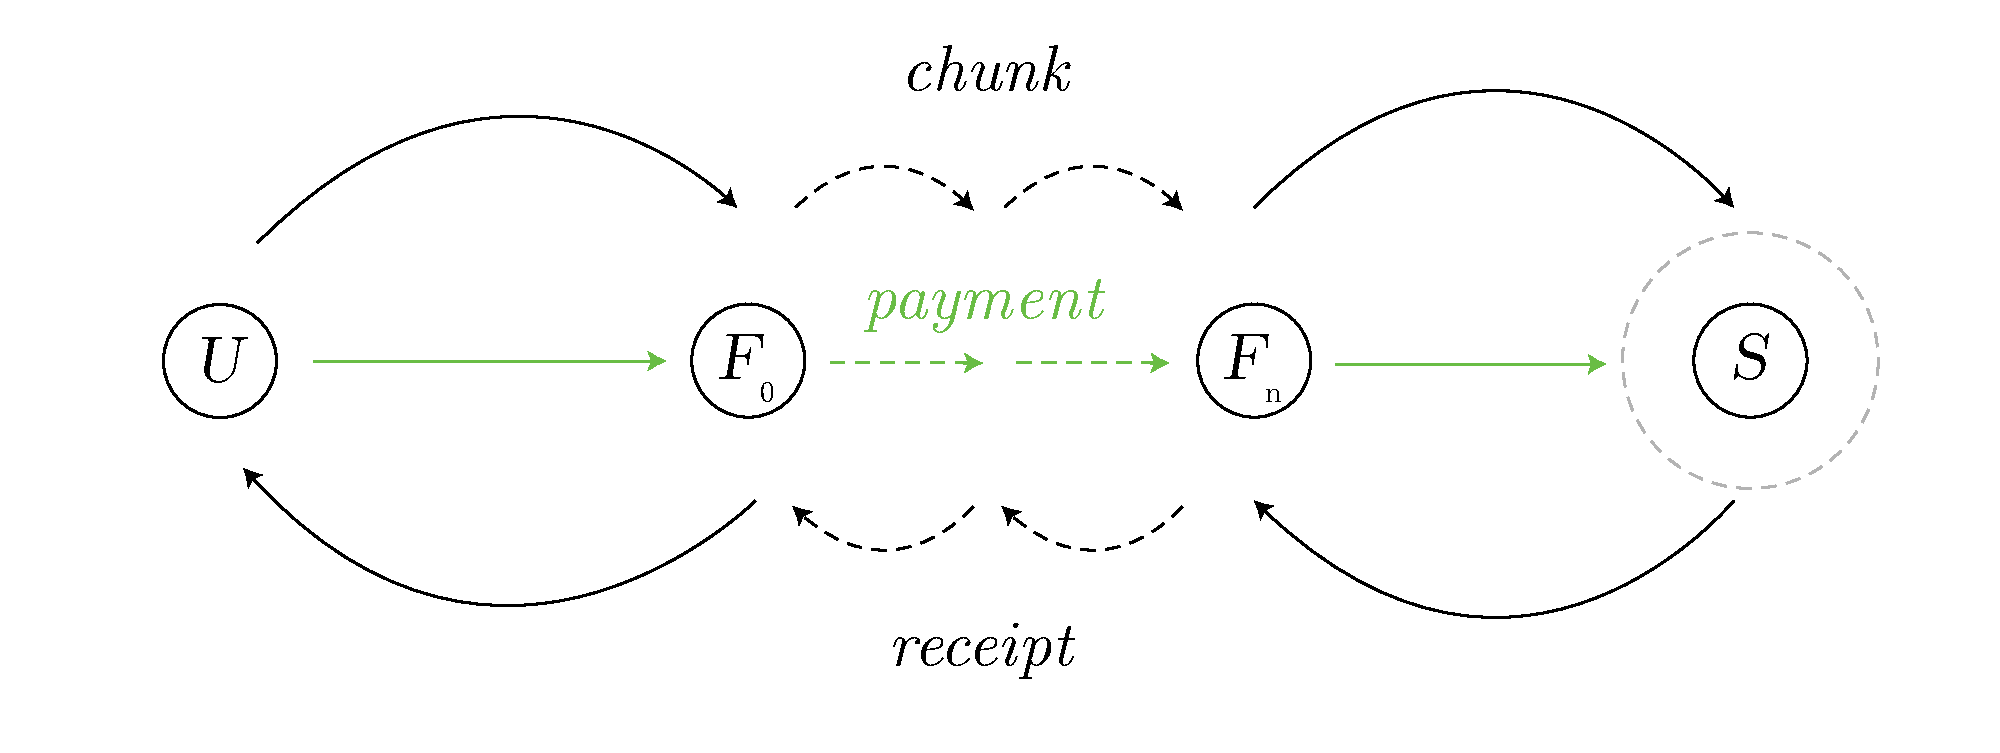
\includegraphics[width=0.8\textwidth]{figs/push-payment.pdf}
%   \caption{Incentives for push syncing.}
% \label{fig:push-payment}
% \end{figure}



% How to determine when to forward.
% discuss the cost of a dream

\subsection{Security}


The reference does not leak either the step-count or any other information about the neighbourhoods touched. Neither do the participants in the protocol know which position they are at in the chain or anything  about the other neighbourhoods except for the following one to which they are push-syncing their chunk.

The construction is deniable.
Beside our sensitive content $C$, take $A$, any uncontroversial content chunk. When producing $C'$, the owner also produces  $A'=A\xor k$ and upload it. When asked about $k$, producing $A$ makes the denial of other content including $C$ more plausible. \qedsymbol

% Swarm is a decentralized network where individual participants cannot (and should not) be trusted to play by the rules; it is the built-in incentives that encourage cooperative behavior and help maintain it, it being a Nash-equilibrium. The condition for content deletion to be achieved is that in \emph{at least one neighborhood} all nodes are honest, i.e., do not operate a malicious node which would store and serve information that they should not store and serve.% 
% %
% \footnote{With the growth of the Swarm network, the number of neighborhoods increases whereas the membership of neighborhoods remains about the same. Thus, the costs of attacking the proposed scheme are expected to increase with network size.}
% %

A powerful adversary can infiltrate every neighborhood of Swarm and archive all information that has ever been uploaded (without being able to decipher it surely) and keep logs of what has been uploaded in what order, which would allow it to serve up deleted content on demand. But there is a huge price on such indiscriminate archiving of all Swarm's content and that is the only way to reliably defeat the dream construction.

We now turn to the discussion how to calibrate the step-count given a security model. Let us assume a network-wide neighbourhood infiltration rate of $\frac{1}{2}$, meaning that  half of the neighbourhoods in the network is assumed  to be  malicious and colluding. 

Assuming that when  revoking access, the owner uploaded new chunks in each neighbourhood on the dream path. 
Given a particular dream chain, 
However, if even  a single neighbourhood on the dream path is honest they respect the newly arrived chunks and divert the dream path, making it never terminate with the grantee. 

% ZWe assume that malicious nodes are able and willing to disregard these  new chunks and in an attempt to facilitate abuse of revoked access respond to the ream protocol just like  before the revocation. if each  neighbourhood  on  the path is malicious, it is in principle possible that the dream protocol gives the unchanged response, and access is abused, i.e., allowed even though it is revoked.
Thus for  a breach of access to happen, all neighbourhoods must be malicious.
In our security model a neighbourhood is malicious with  uniform and independent probability.  For an overall infiltration rate of 1 out of $k$, the chance of all neighbourhoods on a given random dream path being malicious is $k^{-n}$. For a security requirement of success rate of $\sigma$ "nines", i.e error rate less than $10^{-\sigma}$,  we can formulate the requirement as

\begin{equation}
    \frac{1}{k^n}< \frac{1}{10^{-\sigma}}
\end{equation}
Now, expressing $k$ as $10^\kappa$, taking the logarithm of both sides and multiply by $-1$, we get

\begin{equation}
    n > \frac{\sigma}{\kappa}
\end{equation}

With one in every 10 neighbourhoods being malicious, the dream path must have as many hops as the number of nines expressing the success rate.%
%
\footnote{I.e., with malicious node probability $0.1$, a 6-hop-long path will effectively revoke access wtith certainty of $99.9999\%$.}



% Since these parts are symmetrical, it is somewhat misleading to refer to them as ciphertext and key.  However, in the deletable construct one part will be available via a normal hash reference, this we can call one time pad, while the ephemeral part is called encoded content. 


% There is also a variation that "self-destructs", i.e. that deletes itself upon
% retrieval, but it is important to understand that it is a very fragile
% mechanism with no guarantee that the intended recipient will be able to
% download it even once. It should only be used in settings where the recipient can,
% for a limited time, request re-uploading in case the content gets deleted
% without all its parts reaching the recipient. 



% \begin{definition}[pss encode function]

% \begin{equation}
% \Psi(b,d,c)=\mathit{Trojan}(\mathit{nonce}, \mathit{topic}, \mathit{payload})
% \end{equation}
% where
% \begin{equation}
% \mathit{nonce} = c[0:32]
% \end{equation}
% \begin{equation}
% \mathit{topic} = \tau
% \end{equation}
% \begin{equation}
% \mathit{payload}[0:32] =  b
% \end{equation}
% \begin{equation}
% \mathit{payload}[32:34] = \mathit{bigendian.Uint16}(d)
% \end{equation}
% \begin{equation}
% \mathit{payload}[34:4030] = c[100:4096]
% \end{equation}
% \end{definition}
 